\chapter{LTE-R Implementation and Results}
\label{chapter6}
\section{Overview} 
This chapter outlines the outcomes of the cooperative spectrum sensing using soft and hard decision fusion schemes. The $P_{davg}$ vs $SNR$ plot is generated for both the schemes to compare their performance in a real fading scenario on a hardware test-bed. The data files generated using gnuradio are imported in MATLAB for all sensor nodes and the results are derived. As it is expected soft-fusion schemes outperform hard-fusion scheme but as we go to higher SNRs both the schemes generally converges to the same results. For LTE-R performance analysis we have the plot for K-factor variation inside a tunnel for high speed tunnel. We also generated the ber curves for all three modulation schemes proposed for LTE-R and it is evident from the plots for higher K-values we have good connectivity. As the train moves away from the LCXs slot, the K-factor goes down and bit-error rate increases. Finally, we generated the continuous ber curve to test the performance of LTE-R in a discrete timestep manner.

\section{LTE-R Testbed in Matlab}

We have implemented the simulation testbed in MATLAB, consisting of a transmitter, a channel and a receiver. The K-factor values for the channel model are obtained from Eq.(\ref{kfactor}) and are used to generate a time-series BER curve for different modulation schemes used in LTE-R. The values used for the electrical material properties for tunnel walls~\cite{lter17} and its
specifications are given in Table~\ref{tablelter}. The relative permittivity for the tunnel walls is taken as $\varepsilon_r = 5$ and $\sigma$ is set to 0.1. The simulation is conducted for velocity of $v (Km/h) = $ 300, 400 and 500 Km/h. Since the frequency band allocation for LTE-R will most probably be from 2--6 GHz, hence the $f_c$ values chose are 2, 3 and 5 GHz. The height of the receiver is assumed to be around the length of the train and height of tunnel is chosen as the size of the leaky coaxial cable.

\begin{table*}[t!]
\centering
\caption{Tunnel and Tx/Rx Characteristics}
\begin{tabular}{c  c  c }
   & Dimensions & Simulation Parameters\\\hline
Tunnel & Width = 8.6 m, Height = 7.3 m & $\varepsilon_r = 5$, $\sigma = 0.1~\textrm{Sm}^{-1}$\\\hline
Leaky Feeder Cable (Tx) & Height = 6.1 m & $f_c$ (GHz) = 2, 3, 5\\\hline
Train (Rx) & Height = 4.2 m &  v (km/h) = 300, 400, 500\\
\hline
\end{tabular}
\label{tablelter}
\end{table*}

\begin{figure}[!ht]
\label{finalblock}
\centering
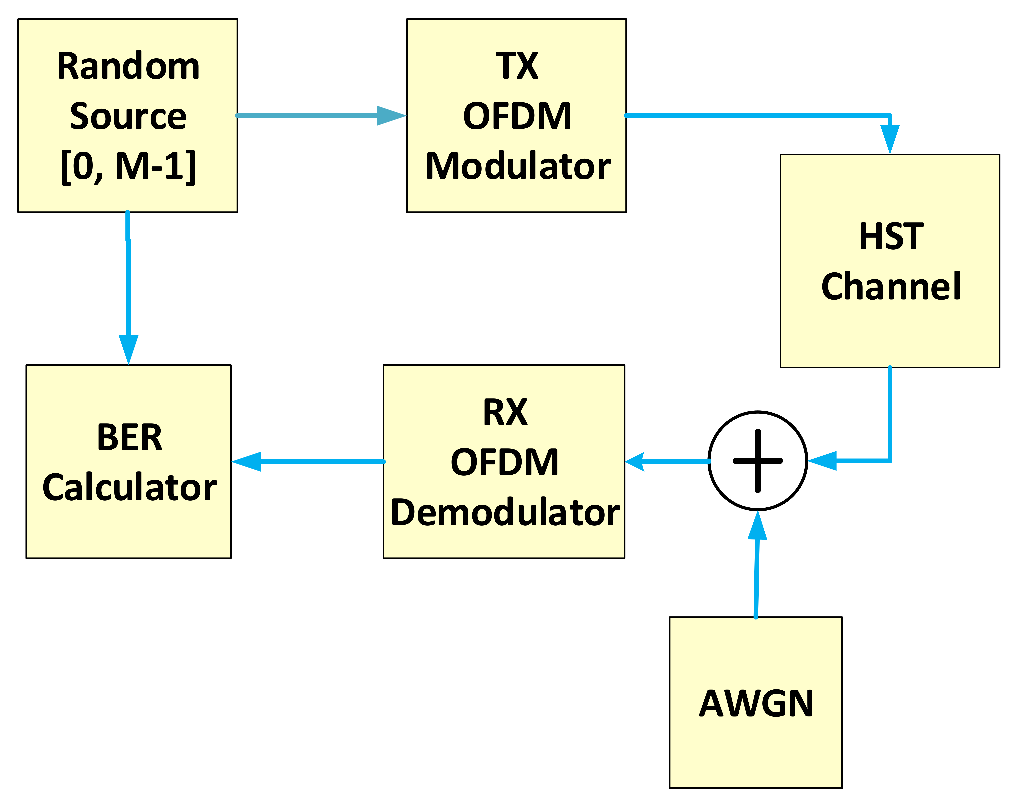
\includegraphics[width=\textwidth,height=8cm,keepaspectratio]{images/Gill/lte_figs/finalblock.eps} 
\caption{Block diagram of a communication system through a HST channel using QPSK, 16-QAM and 64-QAM.}
\end{figure}

Figure~\ref{finalblock} shows the block diagram of the simulation test-bed used for the performance analysis of LTE-R. The random source block generate the symbol between 0 and M-1, where M = 4,16,64 for QPSK, 16QAM and 64QAM respectively. The data is then modulated with specific modulation type and then pass through the proposed HST channel model. The additive white gaussian noise is added after applying the channel coefficients to the signal data. We then demodulate the data packets and pass it to the ber calculator object which then computes the bit-error rate. The simulations are run for SNR values ranging from 0--20 dB and plots are generated for all three modulation schemes.

\section{HST LTE-R in a Tunnel}
Using LTE System Toolbox provided by MATLAB we generated Figure~\ref{lteofdma} which shows the received resource grid without equalization. The frame worth of data was modulated with QPSK, 16QAM and 64QAM for equal number of subcarriers and mapped to symbol in a subframe. We generate ten subframes individually and create one frame after merging all subframes. The frame is passed through our proposed high speed train channel model, with additive white gaussian noise added. We can see that without equalization the received resourced grid has lot of errrors and will lead to numerous retransmissions.

\begin{figure}[!ht]
\label{lteofdma}
\centering
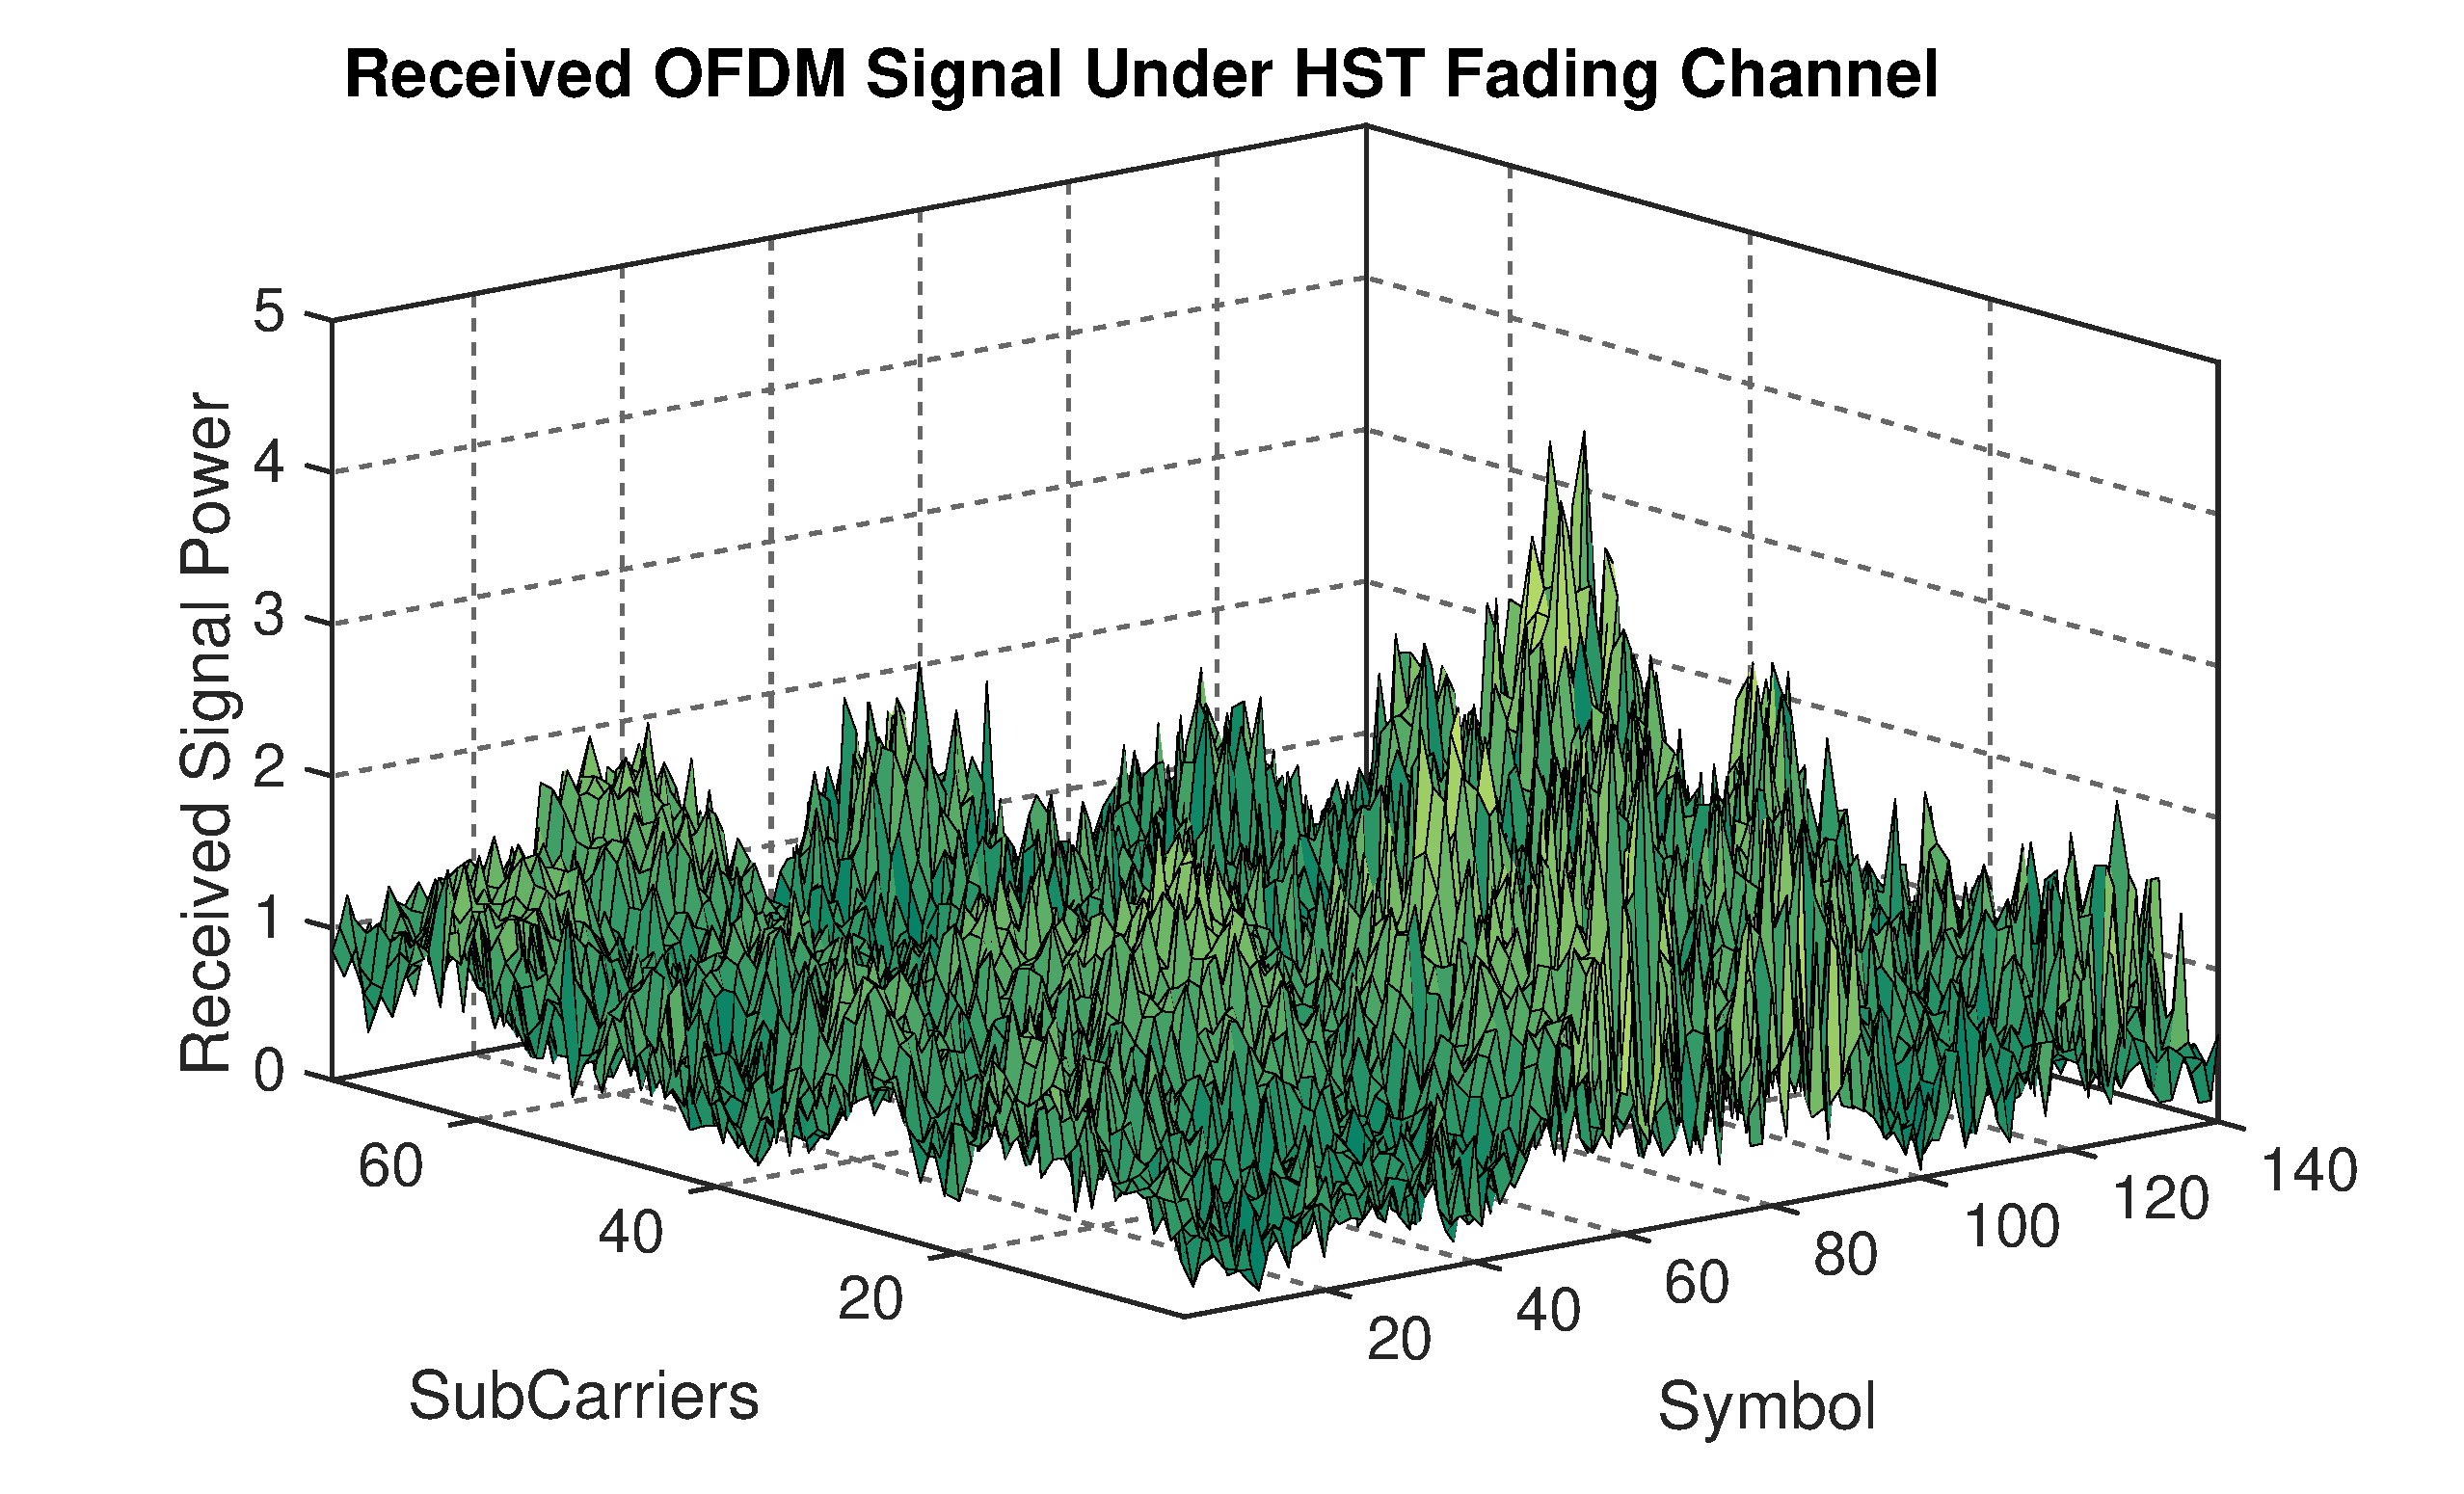
\includegraphics[width=\textwidth,keepaspectratio]{images/Gill/lte_figs/receivedsignal.eps} 
\caption{Received LTE-R OFDM signal under HST Ricean Fading Environment. }
\end{figure}

\subsection{K-factor in a Tunnel}
In Figure~\ref{kfactorber}, we calculated the K-factor for the HST inside a tunnel with velocity $v$ = 500 km/h for different center frequencies. It shows the variation of the Rician K-factor with the distance between the transmitter and receiver as the train is moving along the tunnel. We computed the K-factor for a leaky cable with periodic slots separated by distance d in fixed time-steps. The plot shows that the K-factor varies significantly over a short distances. Therefore, assuming a single K-factor for the channel model is not accurate, we use time-series K-factor to do our channel modeling.

\begin{figure}[!ht]
\label{kfactor}
\centering
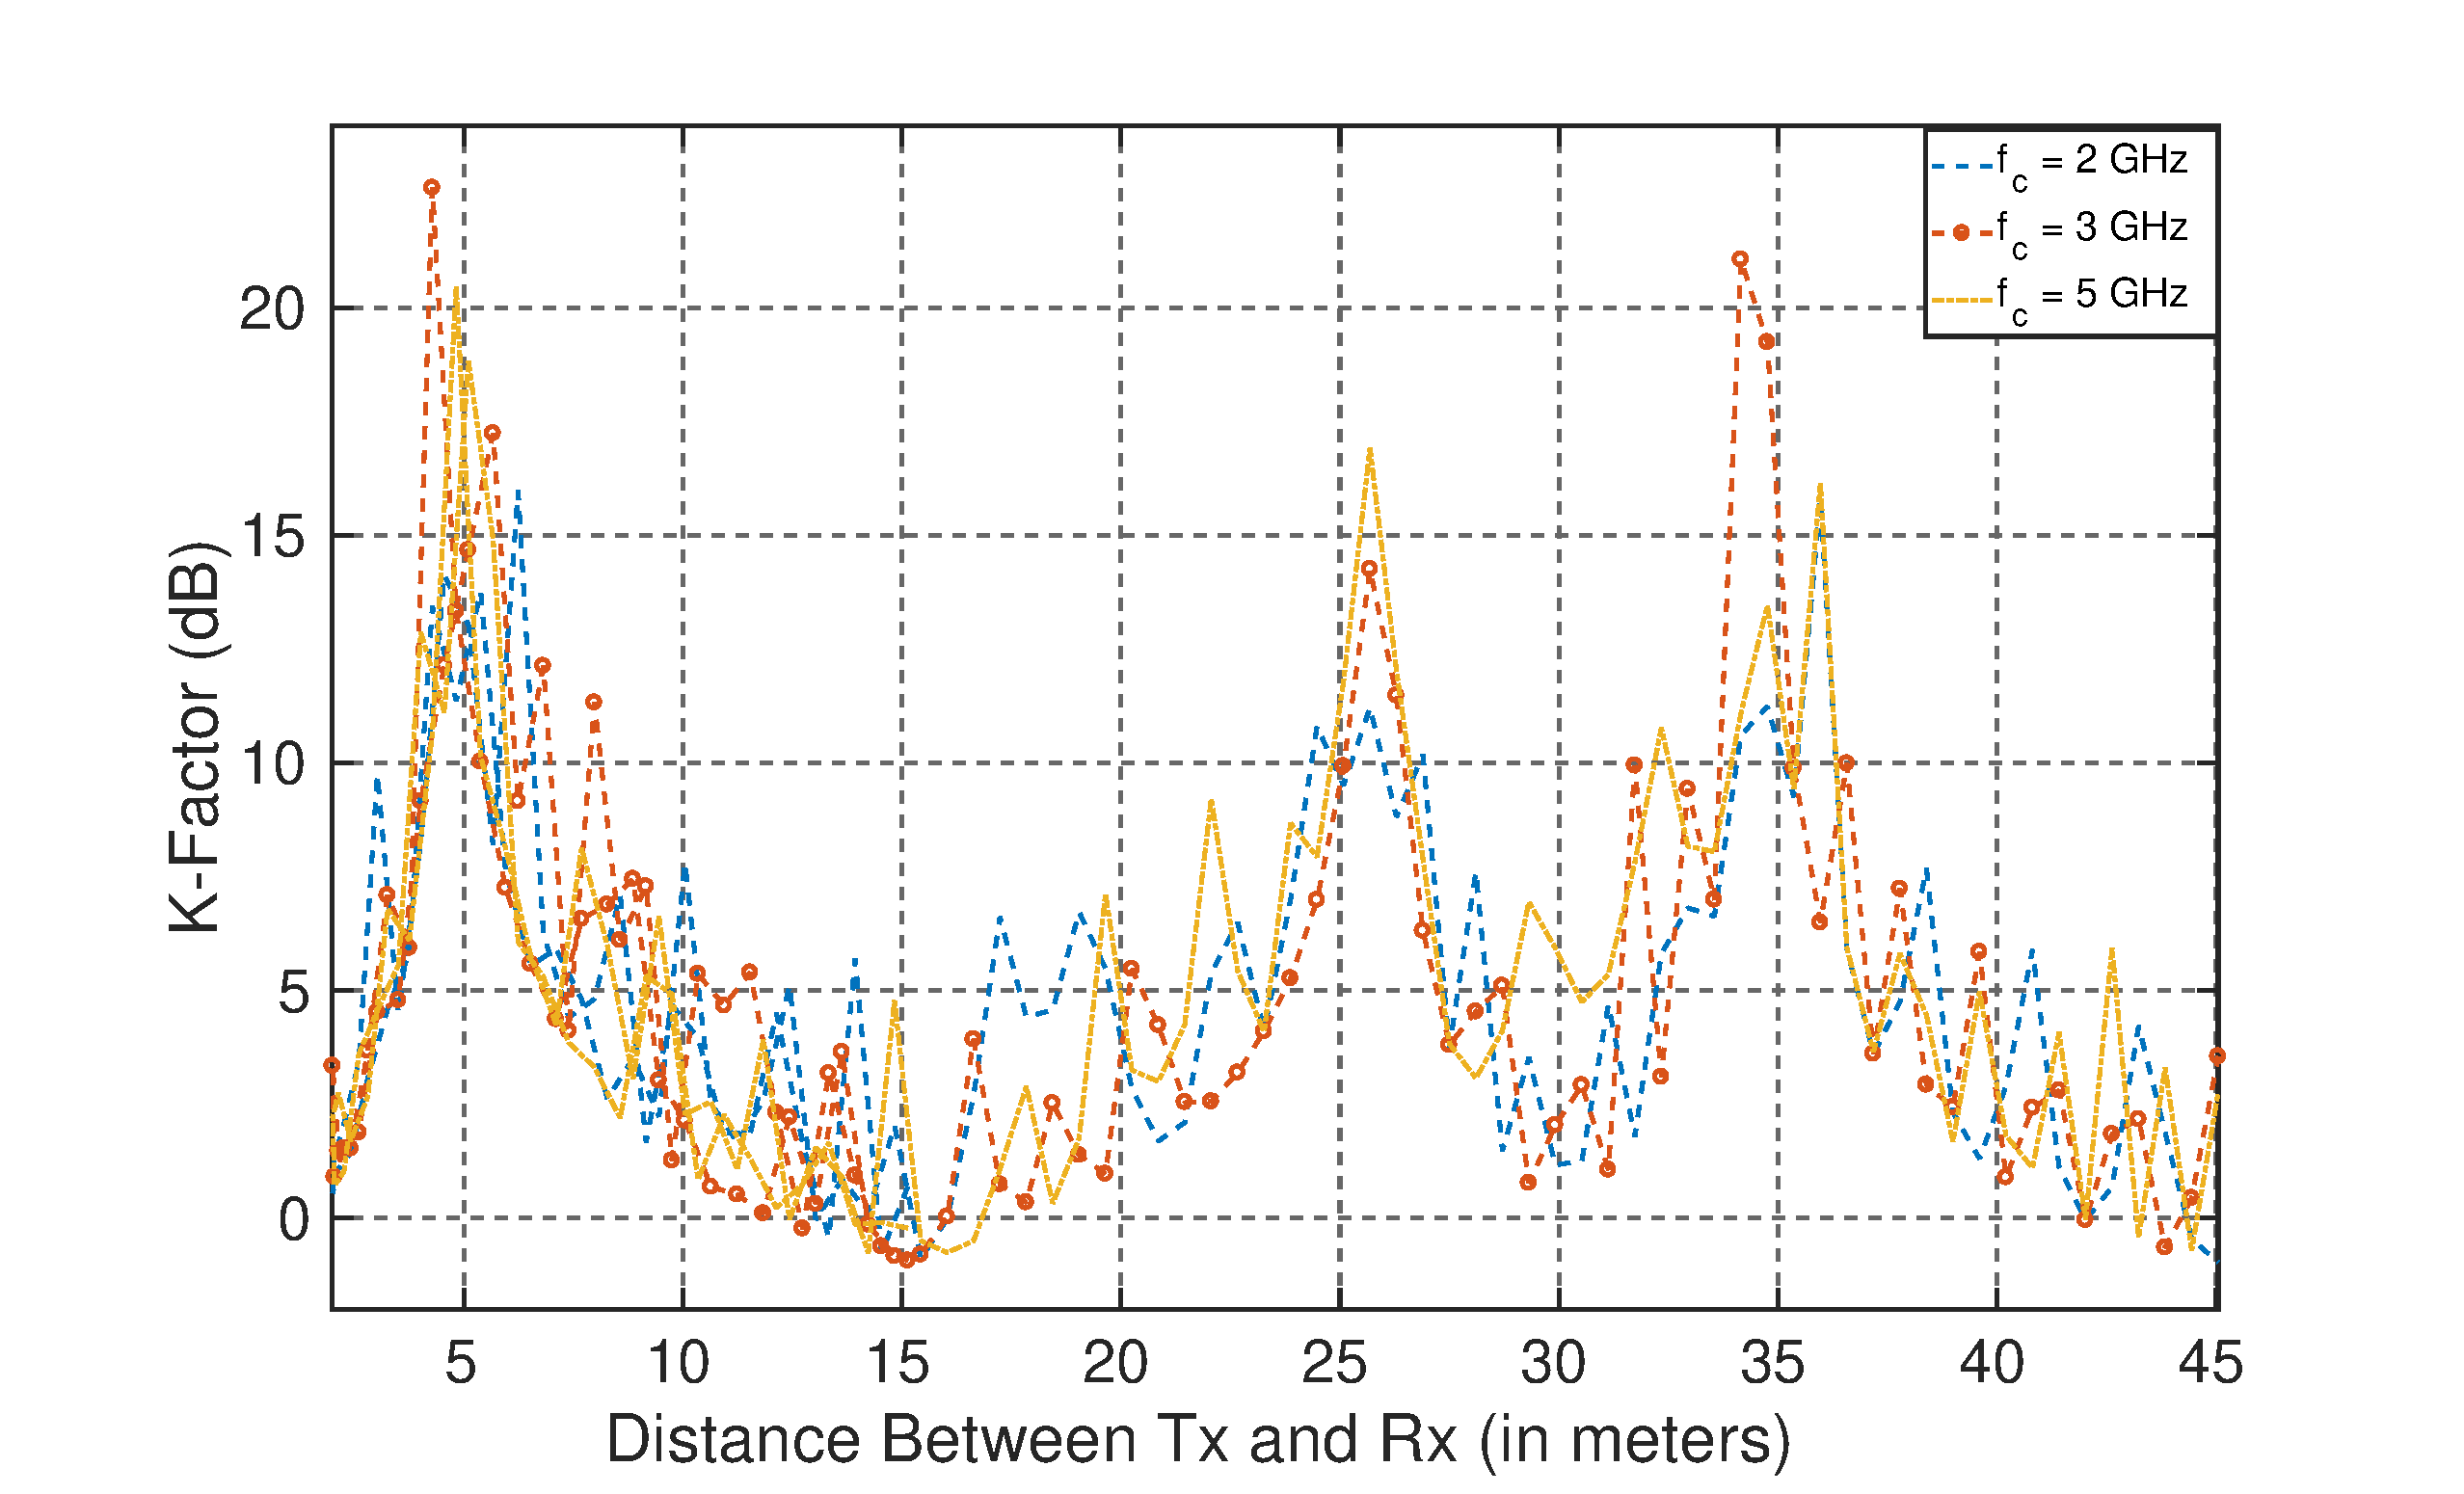
\includegraphics[width=\textwidth,keepaspectratio,height=8cm]{images/Gill/lte_figs/kfactordist.eps} 
\caption{K-factor versus $D_{LOS}$ for different center frequencies $f_c$ = 2, 3 and 5 GHz.}
\end{figure}

\subsection{BER Performance}
To show the impact of varying K-factor on the channel, we computed the BER curve for different modulation schemes of LTE-R with different K-factors. Fig.~\ref{fig:qpsk} shows the BER versus SNR performance for QPSK modulation for different K-factors of the tunnel channel model. The figure clearly demonstrates for higher K-factor we have a better performance while performance degrades as K-factor goes low. Fig.\ref{fig:qam16} shows the $E_b/N_0$ versus BER for 16-QAM and as we can see the BER is higher compared to QPSK. Fig.~\ref{fig:qam64} shows the $E_b/N_0$ versus BER for 64-QAM for different K-factors. And finally we compare all the modulation schemes for the best and worst K-factor in Fig.~\ref{fig:qamall}.

\begin{figure*}[t!]
  \begin{center}
  \subfloat[OFDM-QPSK]
  {\label{fig:qpsk}
  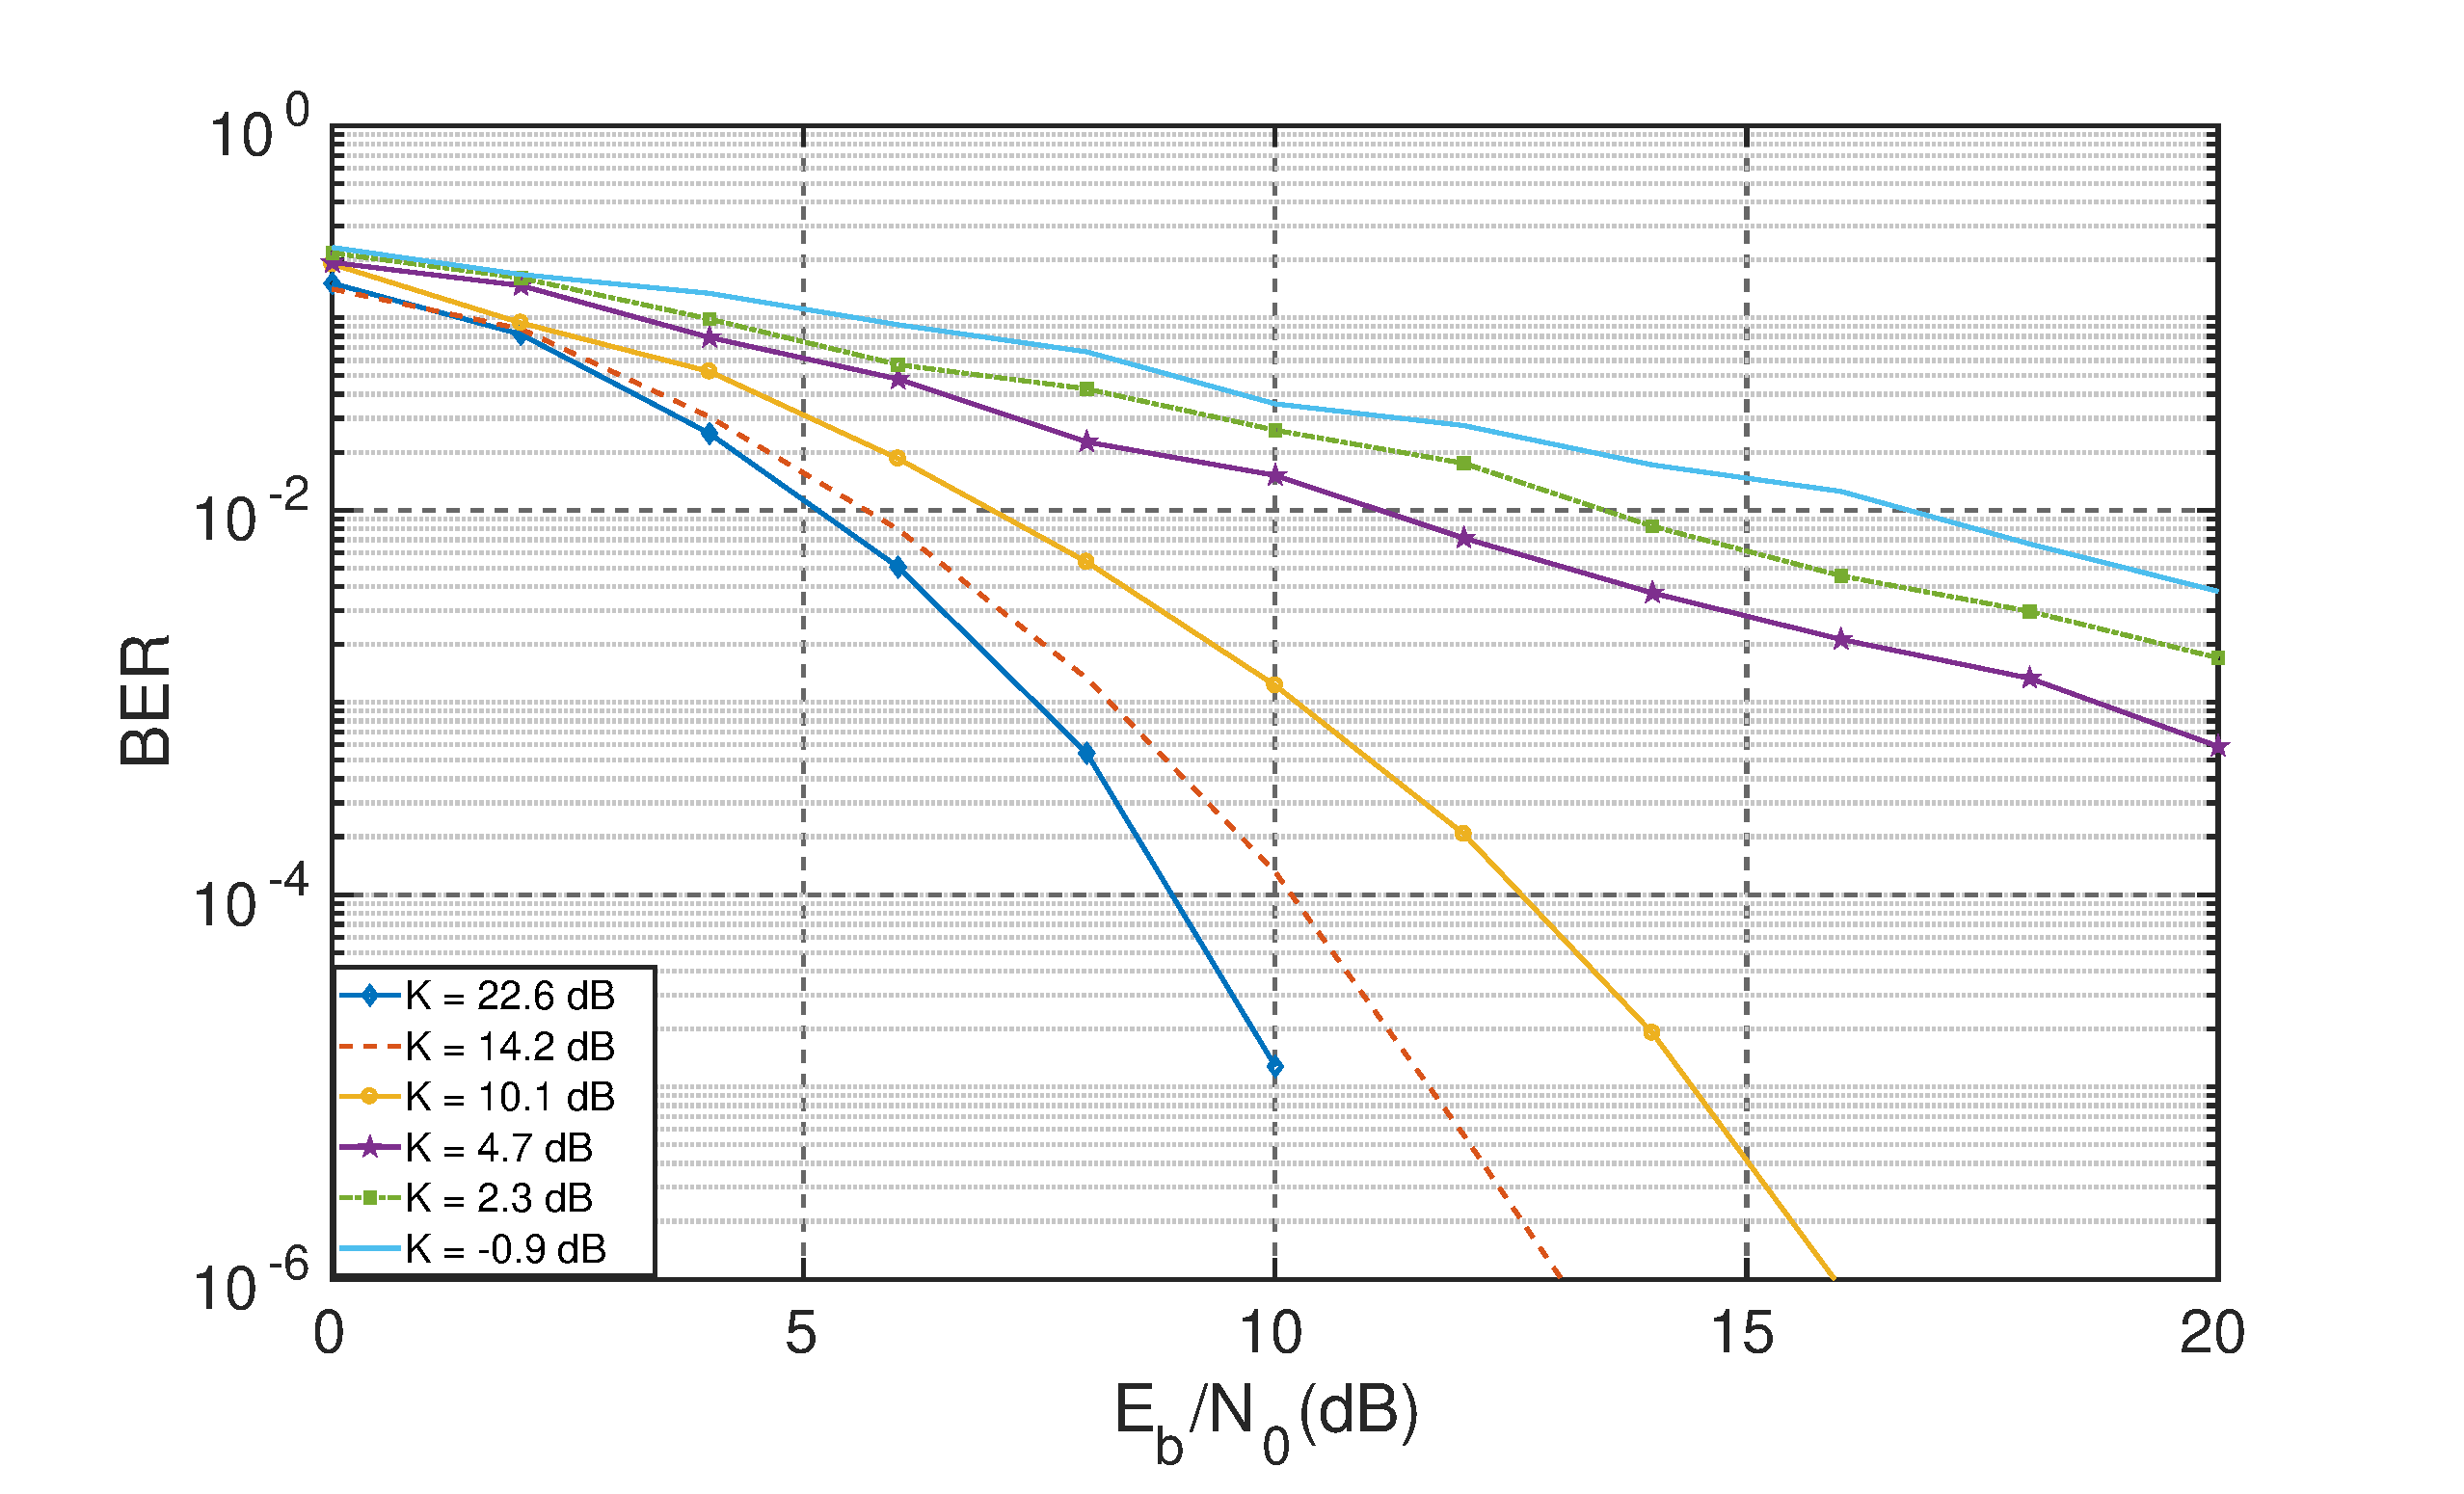
\includegraphics[width=0.46\textwidth]{images/Gill/lte_figs/qpskricean.eps}
  }\hspace{1mm}
   \subfloat[OFDM-16QAM]{\label{fig:qam16}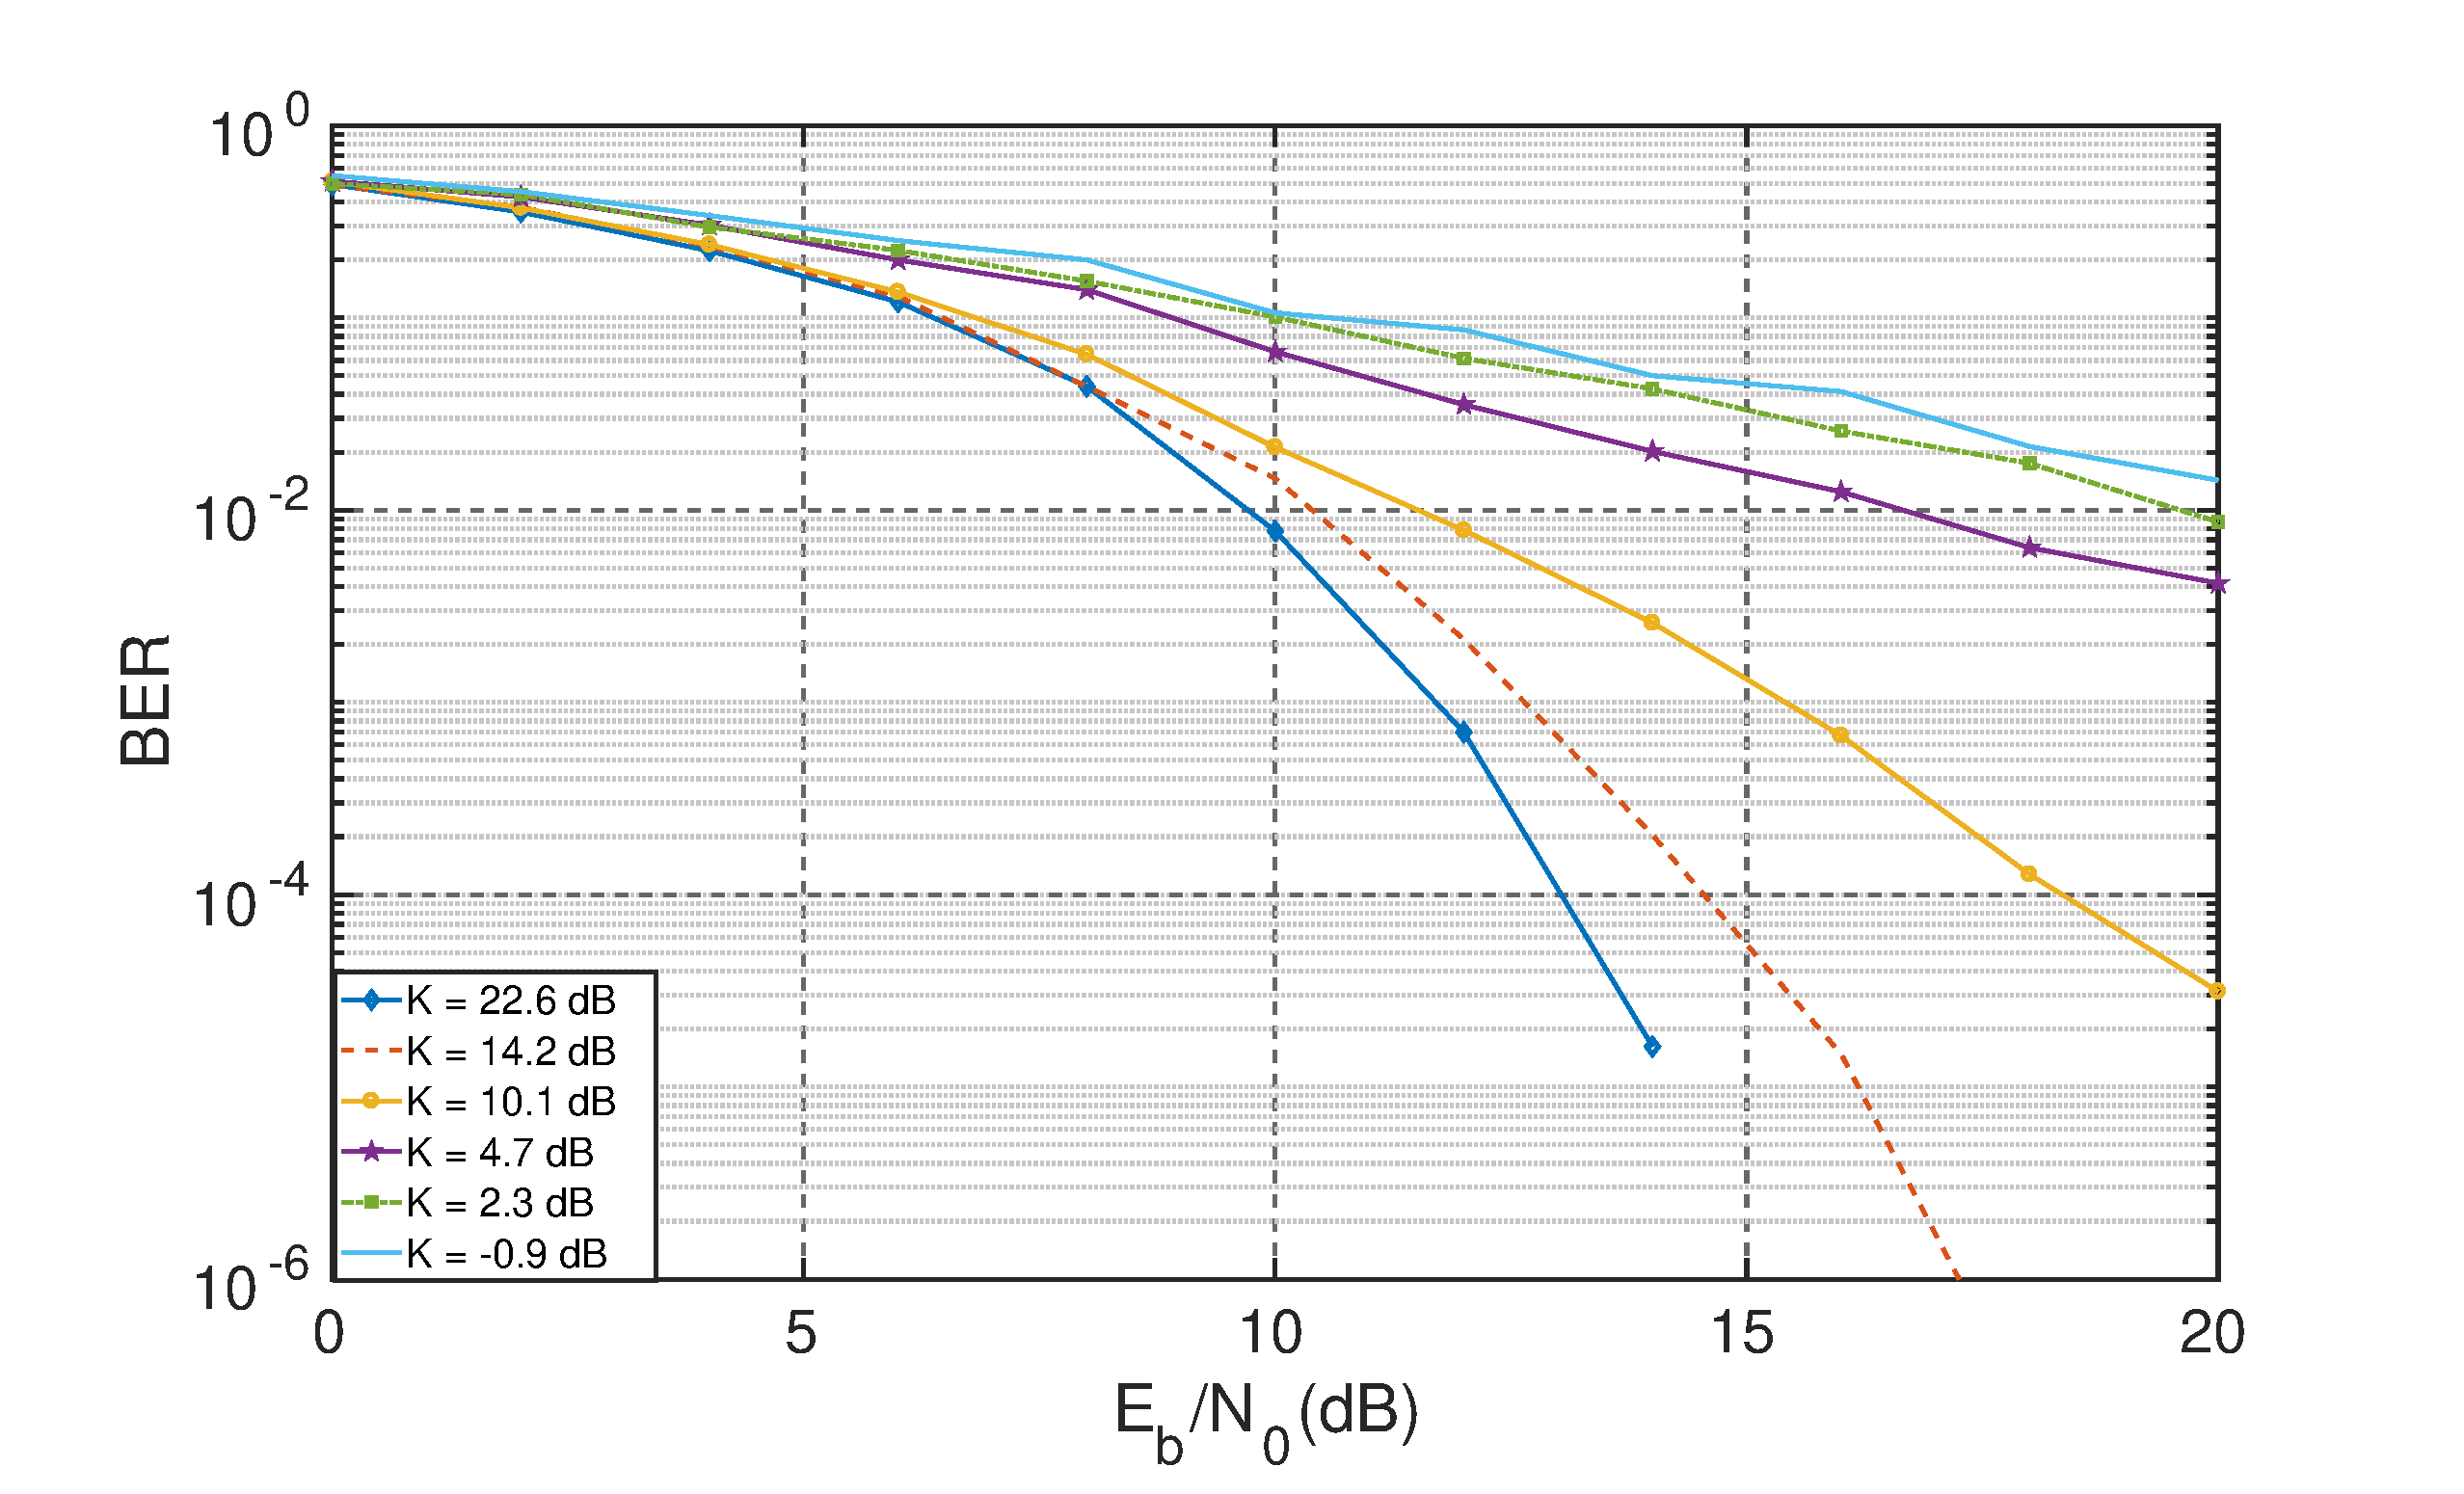
\includegraphics[width=0.46\textwidth]{images/Gill/lte_figs/16qamricean.eps}}\hspace{1mm}
  \subfloat[OFDM-64QAM]{\label{fig:qam64}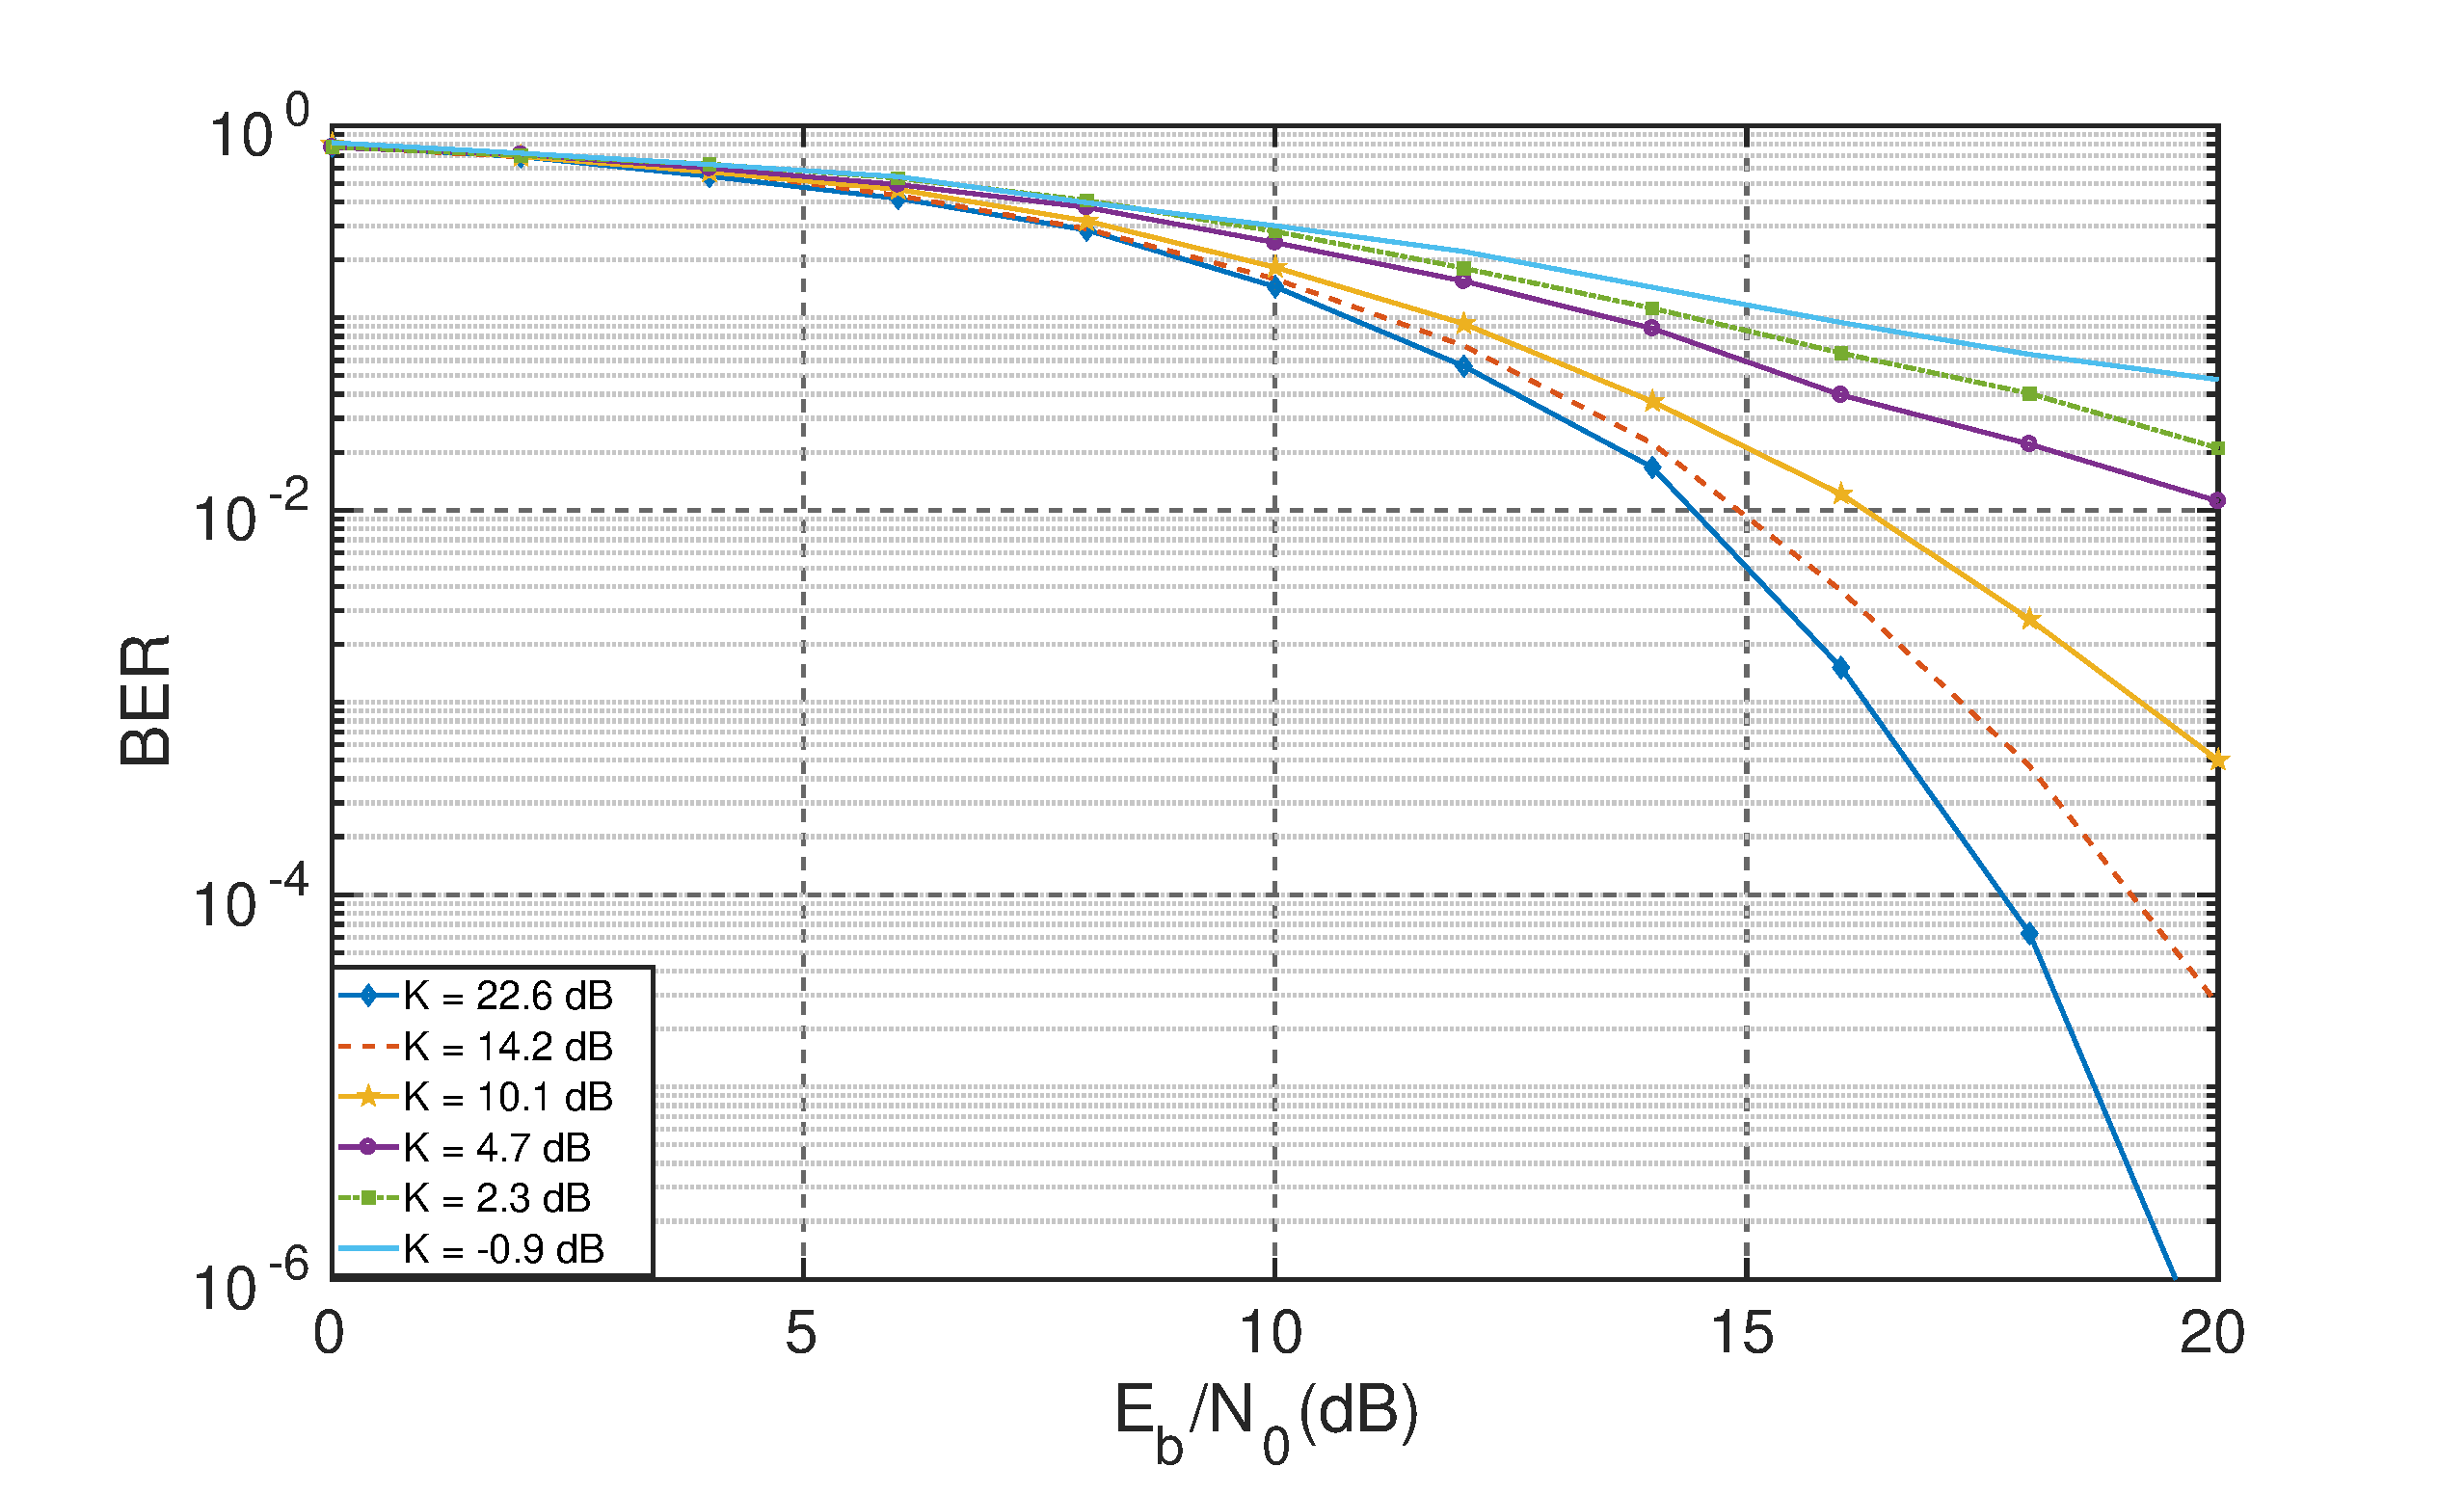
\includegraphics[width=0.46\textwidth]{images/Gill/lte_figs/64qamricean.eps}}\hspace{1mm}
   \subfloat[OFDM-MQAM]{\label{fig:qamall}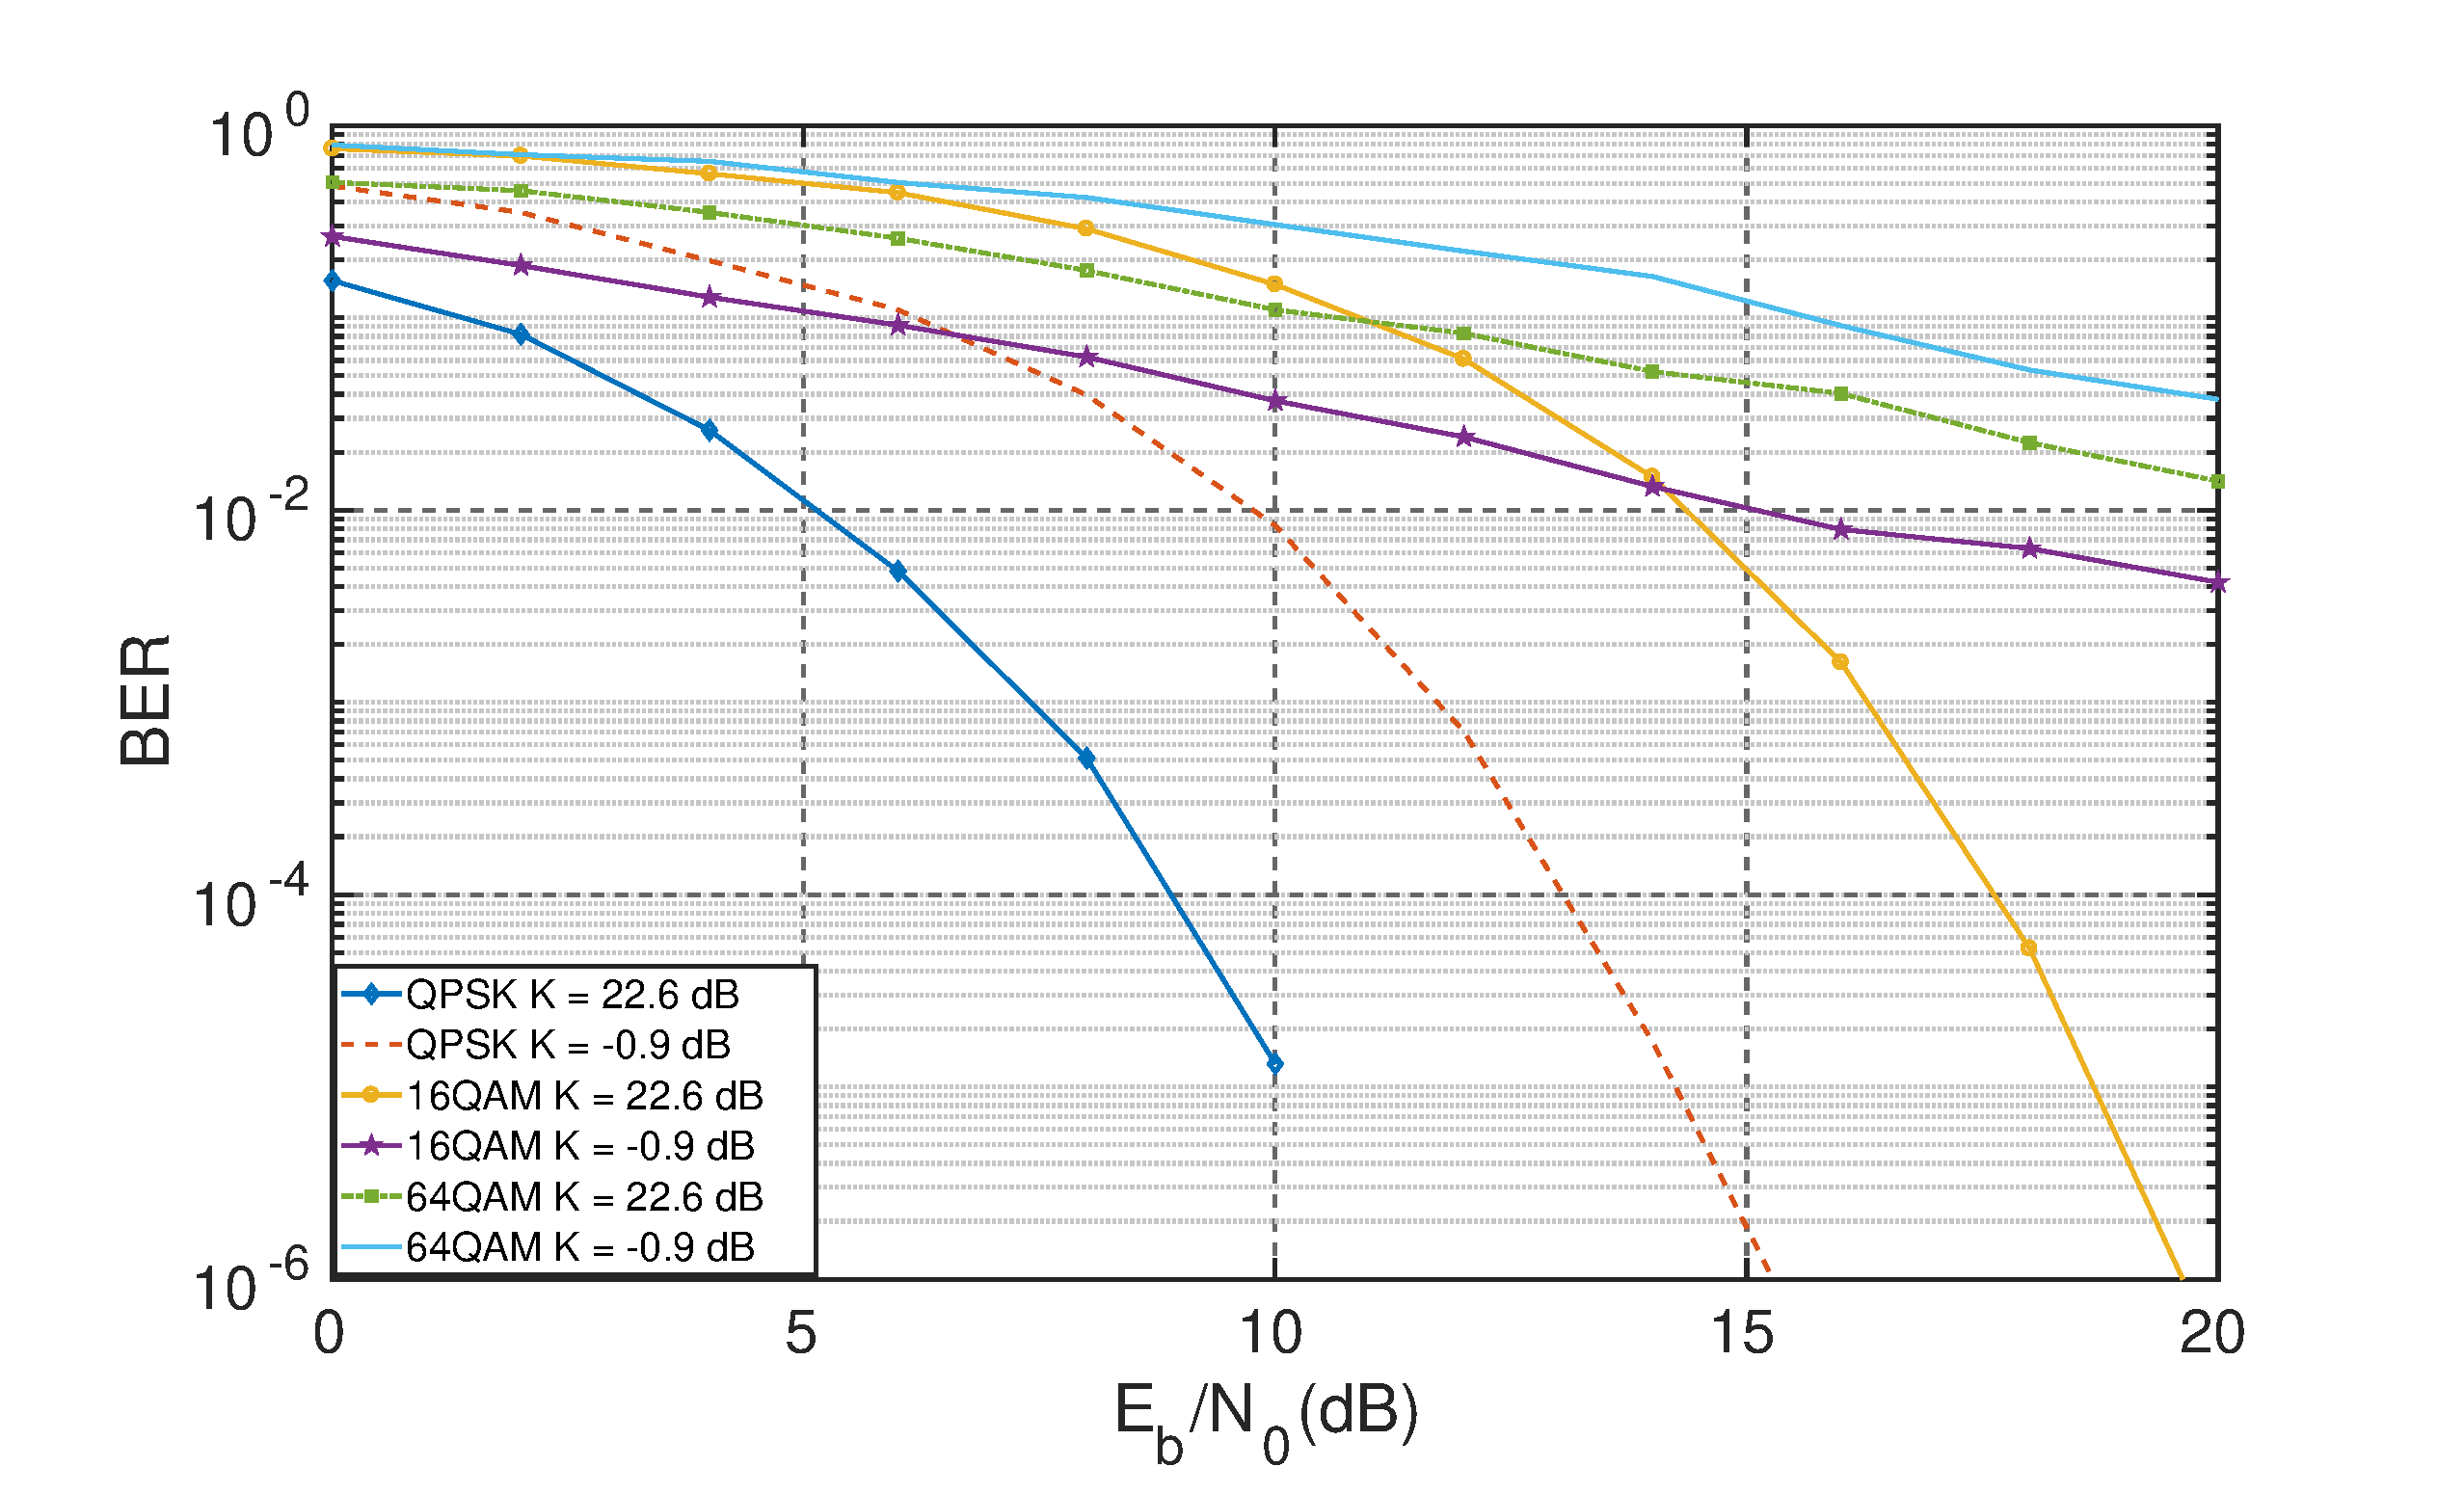
\includegraphics[width=0.46\textwidth]{images/Gill/lte_figs/mqamricean.eps}}\hspace{1mm}
     \caption{Comparison of $E_b/N_0$ verus BER for LTE-R OFDM modulation with different $K$-factors. The first three sub-figures shows the $E_b/N_0$ versus BER for individual modulation schemes employed in LTE-R and in last plot we compare all the modulation schemes for different $K$-factors.} 
\label{fig:modulation}      
   \end{center}
\end{figure*}

In Fig.~\ref{kfactorber} we calculate the BER performance for a high speed train in discrete time-steps. As the train moves towards
the LCX slot the SNR goes high and the SNR decreases as the train moves away. This trend can be seen in the plot, as we move towards the slot the BER curve decreases and it starts increases once we move. It is important to consider here that due to the varying nature of K-factor the BER curve also varies significantly. Hence, by considering the time-varying nature of K-factor we can have a better performance analysis.

\begin{figure}[!ht]
\label{kfactorber}
\centering
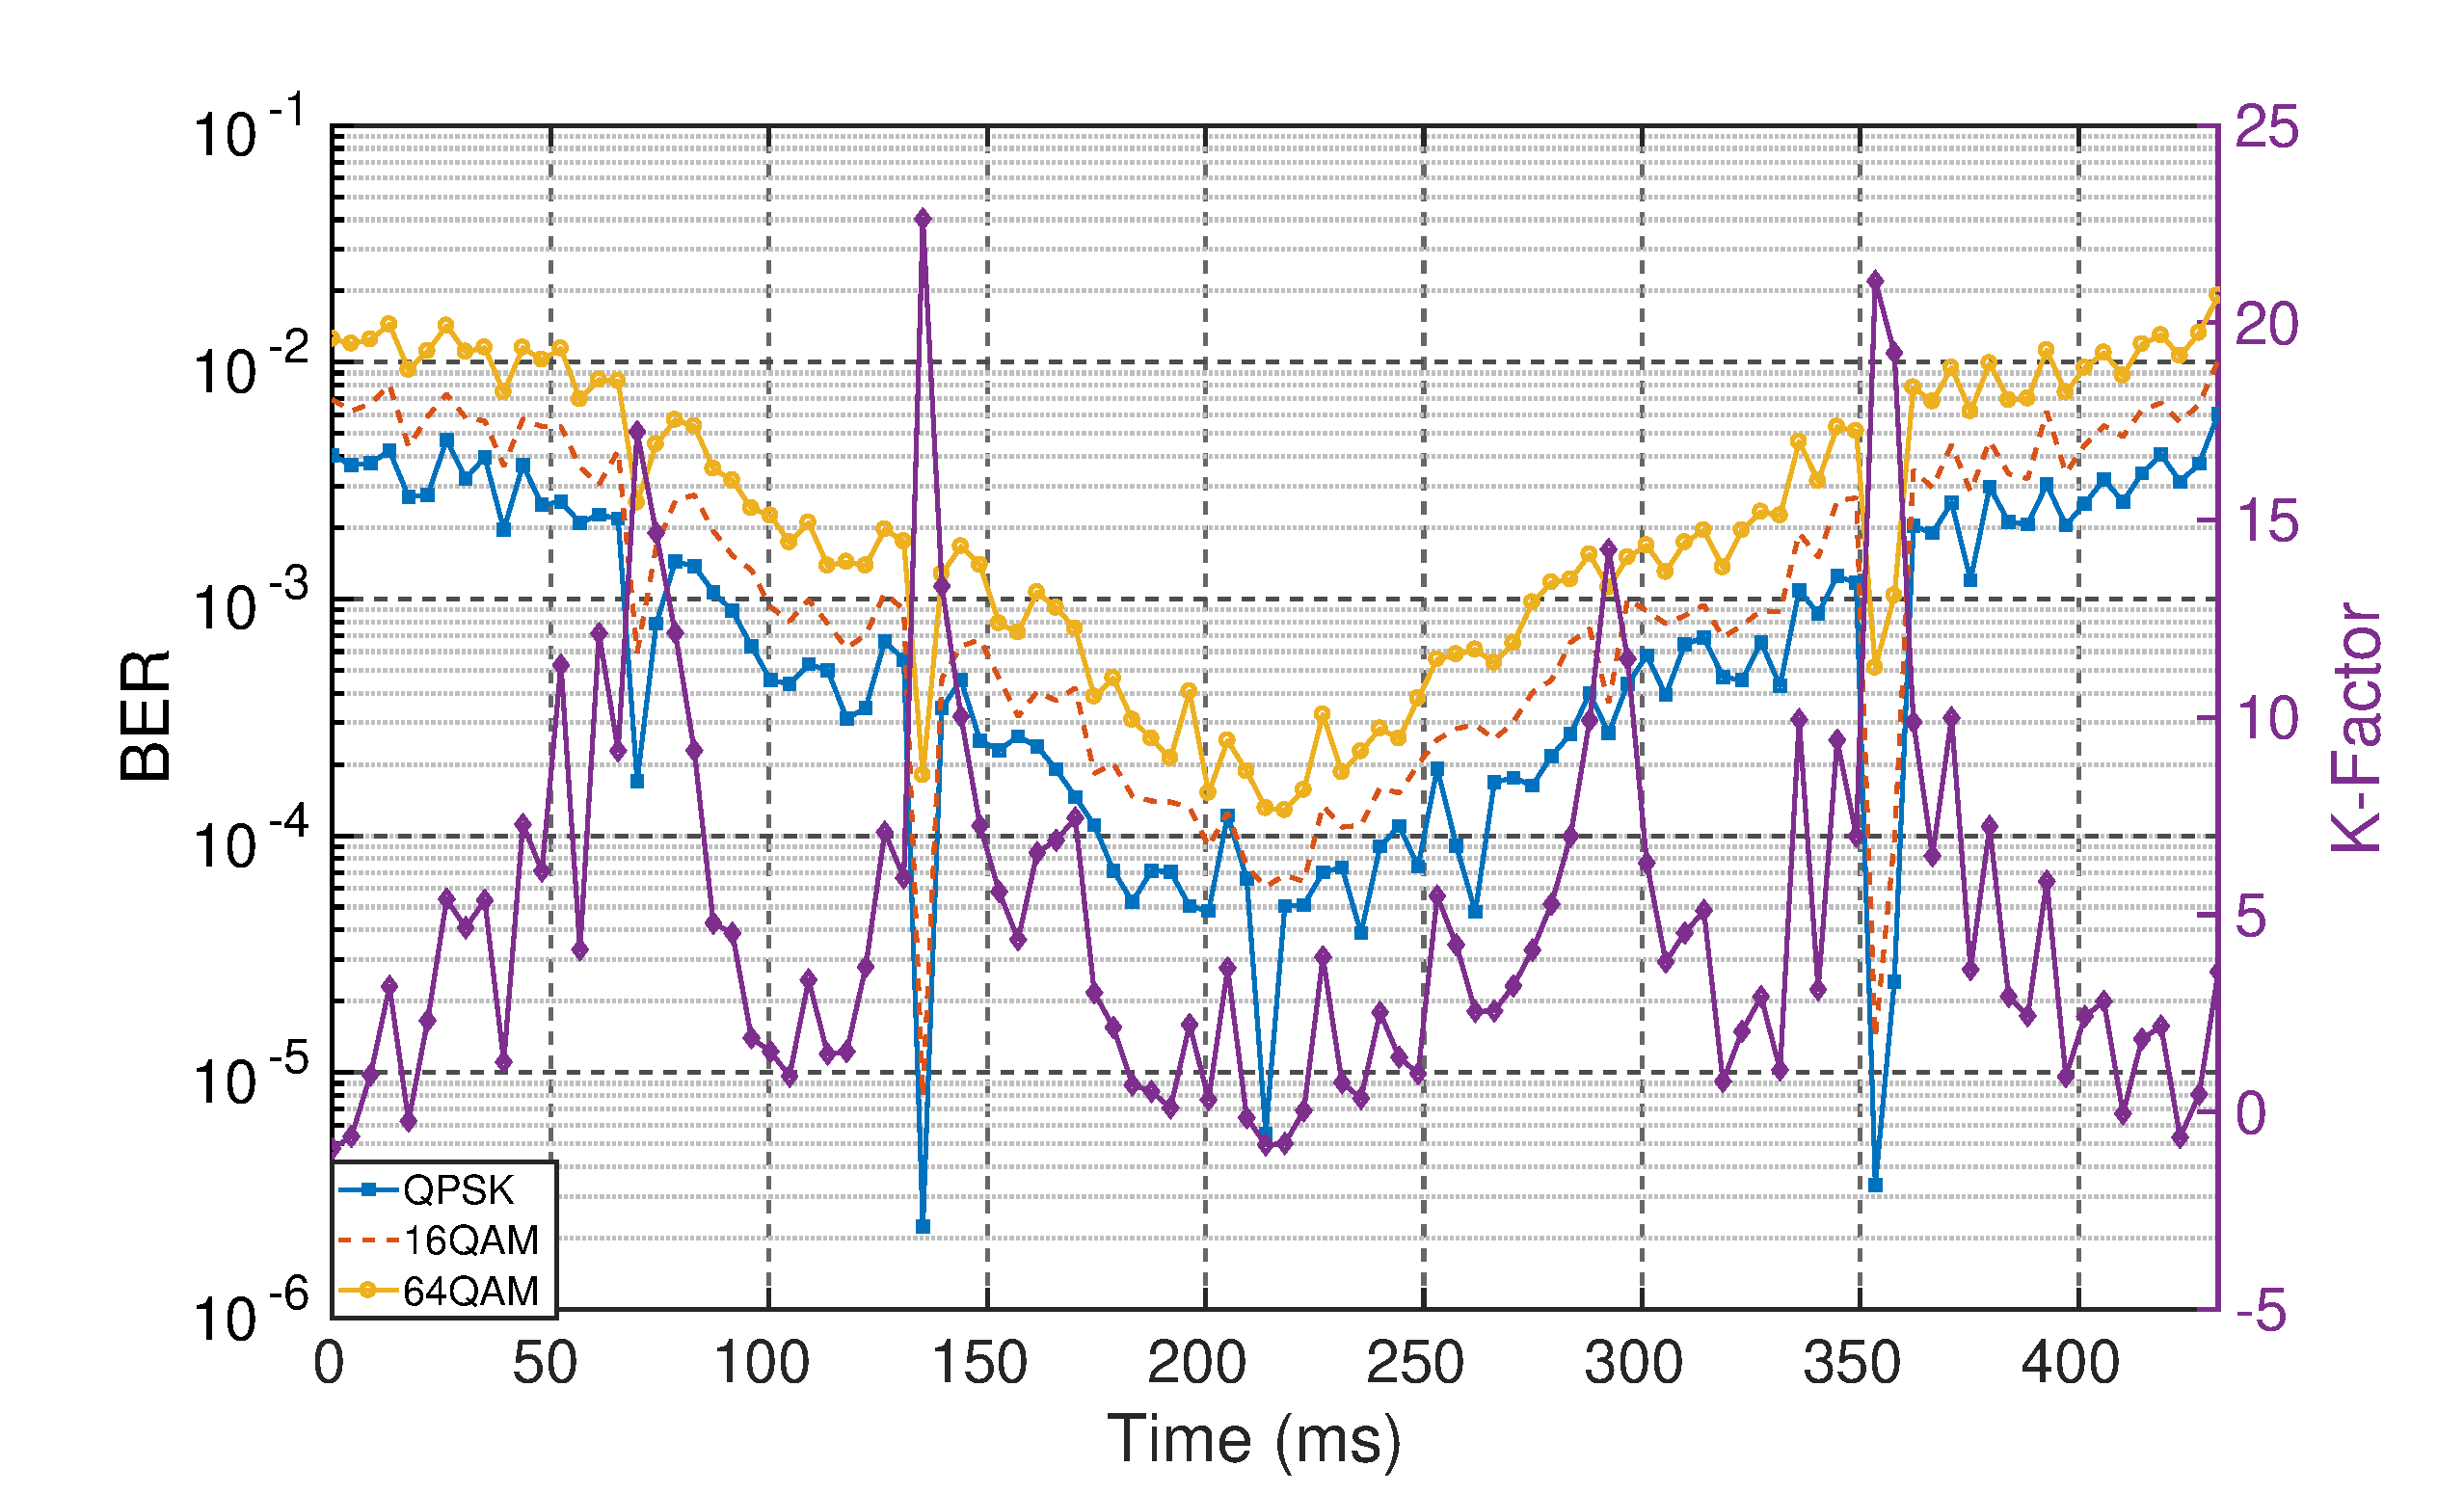
\includegraphics[width=\textwidth,keepaspectratio]{images/Gill/lte_figs/kfactorcontinuous.eps} 
\caption{BER variation with time for HST with different modulation schemes of LTE-R. As the train moves towards
the antenna the general trend of BER goes down with small-scale fluctuations due to varying K-factor.}
\end{figure}

\section{Summary}
We analyzed the BER performance of a LTE-R system for high speed trains inside tunnel environments using our proposed channel model. For the implementation
of our channel, we first derived the time-series K-factor function using the classical two-ray propagation model. We then analyzed the LTE-R performance under our channel model for different modulation schemes for various K-factors. Finally, we compared all the modulation schemes under worst and best K-factor, and we observed that for low $E_b/N_0$
sub-carriers must be modulated with QPSK for maintaining reliable communication link.



